\chapter{Implementing New Features}
\label{cha:newfeatures}
\begin{quote}
First, solve the problem. Then, write the code. --- John Johnson
\end{quote}
\section{Overview}\label{sec:newfeatures-overview}\index{new features}
In this chapter, an example of wil be provided of how to extend \PyPedal{} by creating a user-defined routine.  New routines may implement a new measure of genetic diversity, extend the graphics module, add a new report, or group a series of actions into a single convenient routine.

One of the appealing features of \PyPedal{} is its easy extensibility.  In this section, we will demonstrate how to add a
user-written module to \PyPedal{}.  The file \texttt{pyp\_template.py} that is distributed with \PyPedal{} is a
skeleton that can be used to help you get started writing your custom module(s).  You should also look at the source
code of the standard modules, particularly if there is already a routine that does something similar to what you would
like to do, to see if you can jump-start your project by reusing code.
\subsection{Defining the Problem}
\label{sec:newfeatures-overview-problem}
\index{new features!defining the problem}
Before you open your editor and begin writing code you need to clearly define your problem.  Answering a few questions can
help you do this:
\begin{itemize}
\item What output do I want from my routine?
\item What calculations do I need to perform?
\item What input do I need to give my routine in order to perform those calculations?
\item Are there any \PyPedal{} routines that already do something similar?
\end{itemize}
The last question is as important as the others --- if there is already a \PyPedal{} routine that does similar calculations
you can use it as a starting point.  Code reuse is a great idea.

The problem that will motivate the rest of this section sounds very tricky, but is not really so bad because we are going to
reuse a lot of code.  I want to create a routine for drawing pedigrees that color nodes (animals) based on their importance as
measured by their connectedness to other animals in the pedigree.  After a brief review of the contents of the Module Template
in Section \ref{sec:newfeatures-template}, I will present a detailed solution to this problem in Section
\ref{sec:newfeatures-solving-the-problem}.
\section{Module Template}
\label{sec:newfeatures-template}
\index{new features!module template}
The file \file{pyp\_template.py} is a skeleton that can be used to get started writing a custom module.  The first thing you should do is save a copy of \file{pyp\_template.py} with your working module name; we will use the filename \file{pyp\_jbc.py} for the following example.  You should also fill-in the module header so that it contains your name, e-mail address, etc.  The version number of your module does not have to match that of the main \PyPedal{} distribution, and is only used as an aid to the programmer.
\index{new features!module template!header}
\begin{verbatim}
###############################################################################
# NAME: pyp_jbc.py
# VERSION: 1.0.0 (16NOVEMBER2005)
# AUTHOR: John B. Cole, PhD (jcole@aipl.arsusda.gov)
# LICENSE: LGPL
###############################################################################
# FUNCTIONS:
#     get_color_32()
#     color_pedigree()
#     draw_colored_pedigree()
###############################################################################
\end{verbatim}
The imports section of the template includes \code{import} statements for all of the standard \PyPedal{} modules.  There's
no harm in including all of them in your module, but it's good practice to include only the modules you need. You should
always include the \module{logging} module because it's needed for communicating with the log file.  For \module{pyp\_jbc}
I am including only the \module{pyp\_graphics}, \module{pyp\_network}, and \module{pyp\_utils} modules.
\index{new features!module template!imports}
\begin{verbatim}
##
# pyp_jbc provides tools for enhanced pedigree drawing.
##
import logging
from PyPedal import pyp_graphics
from PyPedal import pyp_network
from PyPedal import pyp_utils
\end{verbatim}
There is a very sketchy function prototype included in the template.  It is probably enough for you to get started if you have
a little experience programming in Python.  If you don't have any experience programming in Python you should be able to get
up-and-running with a little trial-and-error and some study of \PyPedal{} source.  You should always write a comment block similar to that attached to \function{yourFunctionName()} for each of your functions.  This comment block is recognized by PythonDoc, a tool for automatically generating program documentation.  Parameters are the inputs that you send to a function, return is a description of the function's output, and defreturn is the type of output that is returned, such as a list, dictionary, integer, or tuple.
\index{new features!module template!function prototype}
\begin{verbatim}
##
# yourFunctionName() <description of what function does>
# @param <parameter_name> <parameter description>
# @return <description of returned value(s)
# @defreturn <type of returned data, e.g., 'dictionary' or 'list'>
def yourFunctionName(pedobj):
    try:
        # Do something here
        logging.info('pyp_template/yourFunctionName() did something.')
        # return a value/dictionary/etc.
    except:
        logging.error('pyp_template/yourFunctionName() encountered a problem.')
        return 0
\end{verbatim}
\section{Solving the Problem}
\label{sec:newfeatures-solving-the-problem}
\index{new features!solving the problem}
The measure of connectedness I am going to use for coloring the pedigree is the proportion of animals in the pedigree that are descended from each animal in the pedigree.  In order to do this we need to do the following:
\begin{enumerate}
\item Compute the proportion of animals in the pedigree that are descended from each animal in the pedigree; the values will
be stored in a dictionary keyed by animal IDs.
\item Map the proportion of descendants from decimal values on the interval (0,1) to RGB triples.
\item Use the RGB triples to set the fill color for nodes.
\end{enumerate}
There is not an existing function for the first item, but there is a function in the \module{pyp\_network} module, \function{find_descendants()}, for identifying all of the descendants of an animal.  We can use the length of the list of descendants and the number of animals in the pedigree to calculate the proportion of animals in the pedigree descended from that animal.  The \function{color\_pedigree()} function creates a dictionary and loops over the pedigree to compute the proporions.  It also calls \function{draw\_colored\_pedigree()}, which is a modified version of \function{pyp\_graphics.draw\_pedigree()}, to draw the pedigree with colored nodes.
\begin{verbatim}
##
# color_pedigree() forms a graph object from a pedigree object and
# determines the proportion of animals in a pedigree that are
# descendants of each animal in the pedigree.  The results are used
# to feed draw_colored_pedigree().
# @param pedobj A PyPedal pedigree object.
# @return A 1 for success and a 0 for failure.
# @defreturn integer
def color_pedigree(pedobj):
    _pedgraph = pyp_network.ped_to_graph(pedobj)
    _dprop = {}
    # Walk the pedigree and compute proportion of animals in the
    # pedigree that are descended from each animal.
    for _p in pedobj.pedigree:
        _dcount = pyp_network.find_descendants(_pedgraph,_p.animalID,[])
        if len(_dcount) < 1:
            _dprop[_p.animalID] = 0.0
        else:
            _dprop[_p.animalID] = float(len(_dcount)) / \
                float(pedobj.metadata.num_records)
    del(_pedgraph)
    _gfilename = '%s_colored' % \
        (pyp_utils.string_to_table_name(pedobj.metadata.name))
    draw_colored_pedigree(pedobj, _dprop, gfilename=_gfilename,
        gtitle='Colored Pedigree', gorient='p', gname=1, gdirec='',
        gfontsize=12, garrow=0, gtitloc='b')
\end{verbatim}
\function{pyp\_graphics.draw\_pedigree()} was copied into \module{pyp\_jbc}, renamed to \function{draw\_colored\_pedigree()}, and modified to draw colored nodes.  Two basic changes were made to accomplish that: the function was altered to accept a dictionary of weights to be used for coloring, and code for actually coloring the nodes was written.  The first change was simply the addition of a new required parameter, \var{shading}, to the function header.  The second step required a little more work.  For each animal in the pedigree, the descendant proportion is looked-up in the shading dictionary, the proportion is passed to \function{get\_color\_32()} and converted into an RGB triple, and the \member{filled} and \member{color} attributes for the node representing that animal are set.  The hardest part of creating this routine was determining where changes should be made when modifying \function{pyp\_graphics.draw\_pedigree()}.
\begin{verbatim}
##
# draw_colored_pedigree() uses the pydot bindings to the graphviz library
# to produce a directed graph of your pedigree with paths of inheritance
# as edges and animals as nodes.  If there is more than one generation in
# the pedigree as determind by the 'gen' attributes of the animals in the
# pedigree, draw_pedigree() will use subgraphs to try and group animals in
# the same generation together in the drawing.  Nodes will be colored
# based on the number of outgoing connections (number of offspring).
# @param pedobj A PyPedal pedigree object.
# @param shading A dictionary mapping animal IDs to levels that will be
#                used to color nodes.
# ...
# @return A 1 for success and a 0 for failure.
# @defreturn integer
def draw_colored_pedigree(pedobj, shading, gfilename='pedigree', \
    gtitle='My_Pedigree', gformat='jpg', gsize='f', gdot='1', gorient='l', \
    gdirec='', gname=0, gfontsize=10, garrow=1, gtitloc='b', gtitjust='c'):

    from pyp_utils import string_to_table_name
    _gtitle = string_to_table_name(gtitle)
    ...
    # If we do not have any generations, we have to draw a less-nice graph.
    if len(gens) <= 1:
        for _m in pedobj.pedigree:
            ...
            _an_node = pydot.Node(_node_name)
            ...
            _color = get_color_32(shading[_m.animalID],0.0,1.0)
            _an_node.set_style('filled')
            _an_node.set_color(_color)
            ...
    # Otherwise we can draw a nice graph.
    ...
        ...
            for _m in pedobj.pedigree:
                ...
                _an_node = pydot.Node(_node_name)
                ...
                _color = get_color_32(shading[_m.animalID])
                _an_node.set_style('filled')
                _an_node.set_color(_color)
                ...
\end{verbatim}
The \function{get\_color\_32()} function is a modified version of \function{pyp\_graphics.rmuller\_get\_color()} that returns RGB triplets of the form \samp{\#1a2b3c}, which are required by the program that renders the graphs.  This is another example of how code reuse can reduce development time.
\begin{verbatim}
##
# get_color_32() Converts a float value to one of a continuous range of colors
# using recipe 9.10 from the Python Cookbook.
# @param a Float value to convert to a color.
# @param cmin Minimum value in array (0.0 by default).
# @param cmax Maximum value in array (1.0 by default).
# @return An RGB triplet.
# @defreturn integer
def get_color_32(a,cmin=0.0,cmax=1.0):
    try:
        a = float(a-cmin)/(cmax-cmin)
    except ZeroDivisionError:
        a=0.5 # cmax == cmin
    blue = min((max((4*(0.75-a),0.)),1.))
    red = min((max((4*(a-0.25),0.)),1.))
    green = min((max((4*math.fabs(a-0.5)-1.,0)),1.))
    _r = '%2x' % int(255*red)
    if _r[0] == ' ':
        _r = '0%s' % _r[1]
    _g = '%2x' % int(255*green)
    if _g[0] == ' ':
        _g = '0%s' % _g[1]
    _b = '%2x' % int(255*blue)
    if _b[0] == ' ':
        _b = '0%s' % _b[1]
    _triple = '#%s%s%s' % (_r,_g,_b)
    return _triple
\end{verbatim}
This change will probably be to rolled into \function{rmuller\_get\_color()} so that the form of the return triplet is user-selectable.

The program \file{new_jbc.py} demonstrates use of the new \function{pyp\_jbc.color\_pedigree()} routine:
\begin{verbatim}
options = {}
options['renumber'] = 1
options['sepchar'] = '\t'
options['missing_parent'] = 'animal0'

if __name__=='__main__':
    options['pedfile'] = 'new_ids2.ped'
    options['pedformat'] = 'ASD'
    options['pedname'] = 'Boichard Pedigree'
    example = pyp_newclasses.loadPedigree(options)
    pyp_jbc.color_pedigree(example)
\end{verbatim}
The resulting colorized pedigree can be seen in Figure \ref{fig:boichard2-pedigree-colorized}.  Each of the nodes is colored
according to the proportion of animals in the complete pedigree descended from a given animal.  Clearly there is still room
for improvement; for example, there is no key provided in the image so that you can see how colors map to proportions.  Implementation
of a key is left as an exercise for the reader.
\begin{figure}
  \begin{center}
    \includegraphics[width=6in]{BoichardPedigreeColored.eps}
    \caption{Colorized version of the pedigree in Figure \ref{fig:new-ids2-pedigree-basic}}
    \label{fig:boichard2-pedigree-colorized}
  \end{center}
\end{figure}
\section{Contributing Code to PyPedal}
\label{sec:newfeatures-overview-contributing-code}
\index{new features!contributing code}
If you would like to contribute your code back to \PyPedal{} please note that it must be licensed under version 2.1 or any
later version of the GNU Lesser General Public License.  The GNU LGPL has all of the restrictions of the GPL except that you
may use the code at compile time without the derivative work becoming a GPL work. This allows the use of the code in
proprietary works.  You must also complete and return the joint copyright assignment form distributed as
\texttt{pypedal\_copyright\_assignment.pdf} before any contributions can be accepted and merged into the development tree.

Contributors are asked to document their code using the documentation comments recognized by PythonDoc 2.0 or later
(\url{http://effbot.org/zone/pythondoc.htm}).  PythonDoc is used to generates API documentation in HTML and other formats
based on descriptions in Python source files.  You are also strongly encouraged to provide example programs abd datasets
with any code submissions.